\documentclass[tikz,border=5pt]{standalone}
\usepackage{tikz}
\usepackage{amsmath}

\begin{document}

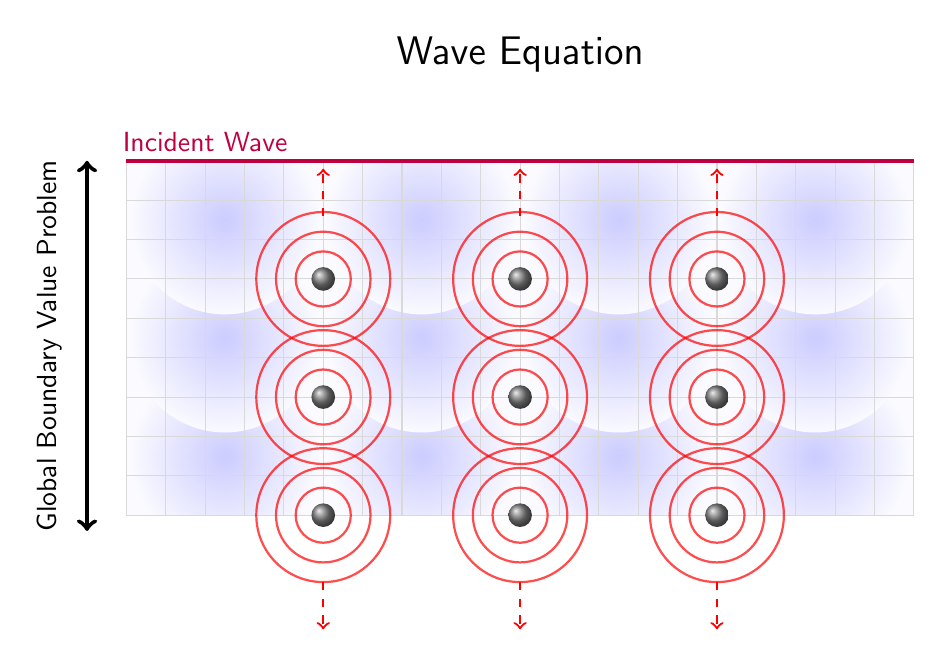
\begin{tikzpicture}[font=\sffamily]
    % Define coordinates for the planes
    \coordinate (TopPlaneLeft) at (0, 3);
    \coordinate (TopPlaneRight) at (10, 3);
    \coordinate (MidPlaneLeft) at (0, 1.5);
    \coordinate (MidPlaneRight) at (10, 1.5);
    \coordinate (BotPlaneLeft) at (0, 0);
    \coordinate (BotPlaneRight) at (10, 0);

    % Title
    \node[anchor=south] at (5, 5.5) {\Large Wave Equation};

    % Visualize the continuous potential / refractive index
    % Same as WPM to show it handles the same medium
    \fill[blue!2] (0,0) rectangle (10, 4.5);
    
    \begin{scope}
        \clip (0,0) rectangle (10, 4.5);
        \foreach \x in {1.25, 3.75, 6.25, 8.75} {
            \foreach \y in {0.75, 2.25, 3.75} {
                 \shade[inner color=blue!20, outer color=blue!2] (\x, \y) circle (1.2);
            }
        }
    \end{scope}

    % Finite Element / Finite Difference Grid
    % Represents that this is solved as a Boundary Value Problem on a mesh, not slice-by-slice
    \draw[step=0.5, gray!30, thin] (0,0) grid (10, 4.5);

    % Atoms / Scattering Centers
    % Same positions as other diagrams
    \foreach \y in {0, 1.5, 3} {
        \foreach \x in {2.5, 5, 7.5} {
            \shade[ball color=gray] (\x, \y) circle (0.15);
            
            % Full Scattering Indication
            % Concentric circles radiating in ALL directions (including back)
            % This distinguishes it from the forward-only methods
            \foreach \r in {0.35, 0.6, 0.85} {
                \draw[red, thick, opacity=0.7] (\x, \y) circle (\r);
            }
        }
    }

    % Backscattering Indication
    % Arrows pointing UP significantly distinguish Helmholtz
    \foreach \x in {2.5, 5, 7.5} {
        \draw[->, red, dashed, thick] (\x, 3.8) -- (\x, 4.4);
        \draw[->, red, dashed, thick] (\x, -0.85) -- (\x, -1.45);
    }

    % Electron Wave Propagation Label
    % Changed to indicate it's a global solution
    \draw[<->, ultra thick, black] (-0.5, 4.5) -- (-0.5, -0.2);
    \node[rotate=90, anchor=south, black] at (-0.7, 2.15) {Global Boundary Value Problem};
    
    % Wavefront line
    \draw[ultra thick, purple] (0, 4.5) -- (10, 4.5);
    \node[purple, anchor=south] at (1, 4.5) {Incident Wave};

\end{tikzpicture}

\end{document}
